\documentclass[11pt,openany]{book}
\usepackage[]{graphicx}\usepackage[]{color}
%% maxwidth is the original width if it is less than linewidth
%% otherwise use linewidth (to make sure the graphics do not exceed the margin)
\makeatletter
\def\maxwidth{ %
  \ifdim\Gin@nat@width>\linewidth
    \linewidth
  \else
    \Gin@nat@width
  \fi
}
\makeatother

\definecolor{fgcolor}{rgb}{0.345, 0.345, 0.345}
\newcommand{\hlnum}[1]{\textcolor[rgb]{0.686,0.059,0.569}{#1}}%
\newcommand{\hlstr}[1]{\textcolor[rgb]{0.192,0.494,0.8}{#1}}%
\newcommand{\hlcom}[1]{\textcolor[rgb]{0.678,0.584,0.686}{\textit{#1}}}%
\newcommand{\hlopt}[1]{\textcolor[rgb]{0,0,0}{#1}}%
\newcommand{\hlstd}[1]{\textcolor[rgb]{0.345,0.345,0.345}{#1}}%
\newcommand{\hlkwa}[1]{\textcolor[rgb]{0.161,0.373,0.58}{\textbf{#1}}}%
\newcommand{\hlkwb}[1]{\textcolor[rgb]{0.69,0.353,0.396}{#1}}%
\newcommand{\hlkwc}[1]{\textcolor[rgb]{0.333,0.667,0.333}{#1}}%
\newcommand{\hlkwd}[1]{\textcolor[rgb]{0.737,0.353,0.396}{\textbf{#1}}}%
\let\hlipl\hlkwb

\usepackage{framed}
\makeatletter
\newenvironment{kframe}{%
 \def\at@end@of@kframe{}%
 \ifinner\ifhmode%
  \def\at@end@of@kframe{\end{minipage}}%
  \begin{minipage}{\columnwidth}%
 \fi\fi%
 \def\FrameCommand##1{\hskip\@totalleftmargin \hskip-\fboxsep
 \colorbox{shadecolor}{##1}\hskip-\fboxsep
     % There is no \\@totalrightmargin, so:
     \hskip-\linewidth \hskip-\@totalleftmargin \hskip\columnwidth}%
 \MakeFramed {\advance\hsize-\width
   \@totalleftmargin\z@ \linewidth\hsize
   \@setminipage}}%
 {\par\unskip\endMakeFramed%
 \at@end@of@kframe}
\makeatother

\definecolor{shadecolor}{rgb}{.97, .97, .97}
\definecolor{messagecolor}{rgb}{0, 0, 0}
\definecolor{warningcolor}{rgb}{1, 0, 1}
\definecolor{errorcolor}{rgb}{1, 0, 0}
\newenvironment{knitrout}{}{} % an empty environment to be redefined in TeX

\usepackage{alltt}
\newcommand{\SweaveOpts}[1]{}  % do not interfere with LaTeX
\newcommand{\SweaveInput}[1]{} % because they are not real TeX commands
\newcommand{\Sexpr}[1]{}       % will only be parsed by R


\usepackage[utf8]{inputenc} 
\usepackage{amssymb, amsmath, amsthm}
\usepackage{fullpage}
\usepackage{setspace}
\usepackage{graphicx}
\usepackage{natbib}
\usepackage{rotating}
\usepackage{caption}
\usepackage{subcaption}
\usepackage{multirow}
\usepackage{booktabs}
\usepackage{dcolumn}
\usepackage[grey]{quotchap}
\usepackage{xcolor}
\usepackage[left=1in, top=1in, right=1.5in, bottom=1in, headsep=.5in]
{geometry}
\usepackage{fancyhdr, blindtext}
\usepackage{diagbox}
\usepackage{hyperref} 
\usepackage{placeins}
\renewenvironment{knitrout}{\begin{singlespace}}{\end{singlespace}}
\newcommand*{\mybox}[2]{\colorbox{#1!30}{\parbox{.98\linewidth}{#2}}}
\newcommand*{\befehl}[1]{\texttt{\textbackslash #1}} % Added by 


\fancyhf{}
\fancyhead[LE]{\slshape \rightmark} 
\fancyhead[RE]{\thepage}
\fancyhead[RO]{\slshape \leftmark} 
\fancyhead[LO]{\thepage}
\renewcommand{\headrulewidth}{0.4pt}
\pagestyle{fancy}
%% new command for greybox
\long\def\greybox#1{%
    \newbox\contentbox%
    \newbox\bkgdbox%
    \setbox\contentbox\hbox to \hsize{%
        \vtop{
            \kern\columnsep
            \hbox to \hsize{%
                \kern\columnsep%
                \advance\hsize by -2\columnsep%
                \setlength{\textwidth}{\hsize}%
                \vbox{
                    \parskip=\baselineskip
                    \parindent=0bp
                    #1
                }%
                \kern\columnsep%
            }%
            \kern\columnsep%
        }%
    }%
    \setbox\bkgdbox\vbox{
        \pdfliteral{0.85 0.85 0.85 rg}
        \hrule width  \wd\contentbox %
               height \ht\contentbox %
               depth  \dp\contentbox
        \pdfliteral{0 0 0 rg}
    }%
    \wd\bkgdbox=0bp%
    \vbox{\hbox to \hsize{\box\bkgdbox\box\contentbox}}%
    \vskip\baselineskip%
}
%% make greybox (grbox) a float
\usepackage{float}
\newfloat{grbox}{thp}{lop}[section]
\floatname{grbox}{Grey Box}



\begin{document}





\chapter{Association of Variables}

The last chapter focused on the characterization of distributions of a single variable. We now turn to the associations between two or more variables. This chapter explores ways to measure and visualize associations between variables.   We start with ways to analyze the relations between nominal and ordinal level variables, using \textbf{cross-tabulation} in \textit{R}. Then, for interval level variables, we examine the use of the measures of the \textbf{covariance} and  \textbf{correlation} between pairs of variables. Next we examine hypothesis testing between two groups, where the focus in on how the groups differ, on average, with respect to an interval level variable. Finally, we discuss scatterplots as a way to visually explore differences between pairs of variables. 

\section{Cross-Tabulation}

To determine if there is an association between two variables measured at the nominal or ordinal levels we use cross-tabulation and a set of supporting statistics.  A cross-tabulation (or just crosstab) is a table that looks at the distribution of two variables simultaneously.   Table \ref{tab:IV_DV_Table} provides a sample layout of a 2 X 2 table.

\begin{table}[h]
\centering
\caption{Sample Table Layout} \label{tab:IV_DV_Table}
\begin{tabular}{|l|c|c|c|}
\hline
\diagbox[width=10em]{Dependent\\Variable}{Independent\\Variable} & IV - Low & IV - High & Total \\ \hline
DV - Low & 60\% & 40\% & 53\% \\ \hline
DV - High & 40\% & 60\% & 47\% \\ \hline
 & \begin{tabular}[c]{@{}l@{}}100\%\\ n = 200\end{tabular} & \begin{tabular}[c]{@{}l@{}}100\%\\ n=100\end{tabular} & n = 300 \\ \hline
\end{tabular}
\end{table}

As Table \ref{tab:IV_DV_Table} illustrates, a crosstab is set up so that the independent variable is on the top, forming columns, and the dependent variable is on the side, forming rows.   Toward the upper left hand corner of the table are the low, or negative variable categories.  Generally, a table will be displayed in percentage format.  The marginals for a table are the column totals and the row totals and are the same as a frequency distribution would be for that variable.   Each cross-classification reports how many observations have that shared characteristic.  The cross-classification groups are referred to as \textbf{cells}, so Table \ref{tab:IV_DV_Table} is a four-celled table.

A table like Table \ref{tab:IV_DV_Table} provides a basis to begin to answer the question of whether our independent and dependent variables are related.  Remember that our null hypothesis says there is no relationship between our IV and our DV.  Looking at Table \ref{tab:IV_DV_Table}, we can say of those low on the IV, 60\% of them will also be low on the DV; and that those high on the IV will be low on the DV 40\% of the time.  Our null hypothesis says there should be no difference, but in this case, there is a 20\% difference so it appears that our null hypothesis is incorrect.  What we learned in our inferential statistics chapter, though, tells us that it is still possible that the null hypothesis is true. The question is how likely is it that we could have a 20\% difference in our sample even if the null hypothesis is true?\footnote{To reiterate the general decision rule: if the probability that we could have a 20\% difference in our sample if the null hypothesis is true is less than .05 we will reject our null hypothesis.}

We use the \textbf{chi square statistic} to test our null hypothesis when using crosstabs.  To find chi square ($\chi^2$), we begin by assuming the null hypothesis to be true and find the expected frequencies for each cell in our table.   We do so using a posterior methodology based on the marginals for our dependent variable.   We see that 53\% of our total sample is low on the dependent variable.   If our null hypothesis is correct, then where one is on the independent variable should not matter so 53\% of those who are low on the IV should be low on the DV and 53\% of those who are high on the IV should be low on the DV.  Table \ref{tab:IV_DV_Table2} \& \ref{tab:IV_DV_Table3} illustrate this pattern.  To find the expected frequency for each cell, we simply multiply the expected cell percentage times the number of people in each category of the IV:  the expected frequency for the low-low cell is $.53 * 200 = 106$; for the low-high cell, it is $.47 * 200 = 94$; for the low-high cell it is $.53 * 100 = 53$; and for the high-high cell, the expected frequency is $.47 * 100 = 47$.  (See Table \ref{tab:IV_DV_Table2} \& \ref{tab:IV_DV_Table3})

The formula for the chi square takes the expected frequency for each of the cells and subtracts the observed frequency from it, squares those differences, divides by the expected frequency, and sums those values:

\begin{equation}
  \label{eq:chisquare}
\chi^2  = \sum \frac{(O-E)^2}{E}
  \end{equation}

\noindent where:\\
$\chi^2$  = The Test Statistic\\
$\sum$ = The Summation Operator \\ 
$O$ = Observed Frequencies \\
$E$ = Expected Frequencies \\

\begin{table}[h]
\centering
\caption{ Sample Null-Hypothesized Table Layout as Percentages} \label{tab:IV_DV_Table2}
\begin{tabular}{|l|c|c|c|}
\hline
\diagbox[width=10em]{Dependent\\Variable}{Independent\\Variable} & IV - Low & IV - High & Total \\ \hline
DV - Low & 53\% & 53\% & 53\% \\ \hline
DV - High & 47\% & 47\% & 47\% \\ \hline
 & \begin{tabular}[c]{@{}l@{}}100\%\\ n = 200\end{tabular} & \begin{tabular}[c]{@{}l@{}}100\%\\ n=100\end{tabular} & n = 300 \\ \hline
\end{tabular}
\end{table}

% second tables with values this may need to be combined with previous table.
\begin{table}[h]
\centering
\caption{ Sample Null-Hypothesized Table Layout as Counts} \label{tab:IV_DV_Table3}
\begin{tabular}{|l|c|c|c|}
\hline
\diagbox[width=10em]{Dependent\\Variable}{Independent\\Variable} & IV - Low & IV - High & Total \\ \hline
DV - Low & 106 & 53 & 159 \\ \hline
DV - High & 94 & 47 & 141 \\ \hline
 & 200 & 100 &  300 \\ \hline
\end{tabular}
\end{table}

Table \ref{tab:IV_DV_Table4} provides those calculations.   It shows a final chi square of 10.73.  With that chi square, we can go to a chi square table to determine whether to accept or reject the null hypothesis.  Before going to that chi square table, we need to figure out two things.  First, we need to determine the level of significance we want, presumably .05.  Second, we need to determine our degrees of freedom.  We will have more on that concept as we go on, but for now, know that it is your number of rows minus one times your number of columns minus one.  In this case we have $(2-1)(2-1) = 1$ degree of freedom.  
	 
\begin{table}[h]
\centering
\caption{Chi Square ($\chi^2$) Calculation } \label{tab:IV_DV_Table4}
\begin{tabular}{|l|c|c|c|c|}
\hline
Cell & Observed Freq & Expected Freq & $(O-E)^2$ & $\frac{(O-E)^2}{E}$ \\ \hline
low-low & 120 & 106 & 196 & 1.85 \\ \hline
low-high & 80 & 94 & 196 & 2.09 \\ \hline
high-low & 40 & 53 & 169 & 3.19 \\ \hline
high-high & 60 & 47 & 169 & 3.60 \\ \hline
Total &  &  &  & 10.73 \\ \hline
\end{tabular}
\end{table}

Table \ref{tab:chisquaretable} (at the end of this chapter) is a chi square table that shows the critical values for various levels of significance and degrees of freedom.   The critical value for one degree of freedom with a .05 level of significance is 3.84.  Since our chi square is larger than that we can reject our null hypothesis - there is less than a .05 probability that we could have found the results in our sample if there is no relationship in the population.  In fact, if we follow the row for one degree of freedom across, we see we can reject our null hypothesis even at the .005 level of significance and, almost but not quite, at the .001 level of significance.  

Having rejected the null hypothesis, we believe there is a relationship between the two variables, but we still want to know how strong that relationship is.   Measures of association are used to determine the strength of a relationship. One type of measure of association relies on a co-variation model as elaborated upon in Sections 6.2 and 6.3.  Co-variation models are directional models and require ordinal or interval level measures; otherwise, the variables have no direction.  Here we consider alternative models. 

If one or both of our variables is nominal we cannot specify directional change.  Still, we might see a recognizable pattern of change in one variable as the other variable varies.  Women might be more concerned about climate change than are men, for example. For that type of case, we may use a reduction in error or a \textbf{proportional reduction in error (PRE) model}.  We consider how much better we predict using a naive model (assuming no relationship) and compare it to how much better we predict when we use our independent variable to make that prediction.   These measures of association only range from $0 - 1.0$, since the sign otherwise indicates direction.  Generally, we use this type of measure when at least one our variables is nominal, but we will also use a PRE model measure, $r^2$, in regression analysis.  \textbf{Lambda} is a commonly used PRE-based measure of association for nominal level data, but it can underestimate the relationship in some circumstances. 

Another set of measures of association suitable for nominal level data is based on chi square.  \textbf{Cramer's V} is a simple chi square based indicator, but like chi square itself, its value is affected by the sample size and the dimensions of the table.  \textbf{Phi} corrects for sample size, but is appropriate only for a 2 X 2 table.  The \textbf{contingency coefficient}, C, also corrects for sample size and can be applied to larger tables, but requires a square table, i.e., the same number of rows and columns. 

If we have ordinal level data, we can use a co-variation model, but the specific model developed below in Section 6.3 looks at how observations are distributed around the means.  Since we cannot find a mean for ordinal level data, we need an alternative.  \textbf{Gamma} is commonly used with ordinal level data and provides a summary comparing how many observations fall around the diagonal in the table that supports a positive relationship (e.g. observations in the low-low cell and the high-high cells) as opposed to observations following the negative diagonal (e.g. the low-high cell and the high-low cells).  Gamma ranges from $-1.0$  to $+1.0$.\\

Crosstabulations and their associated statistics can be calculated using R.  In this example we use the Global Climate Change dataset (ds).  The dataset includes measures of survey respondents: gender (female = 0, male = 1); perceived risk posed by climate change or glbccrisk (0 = Not Risk; 10 = extreme risk), and political ideology (1 = strong liberal, 7 = strong conservative). Here we look at whether there is a relationship between gender and the glbccrisk variable.  The glbccrisk variable has eleven categories and to make the table more manageable we recode it to five categories.  

%  time permitting change the variable to age groups.

\begin{knitrout}
\definecolor{shadecolor}{rgb}{0.969, 0.969, 0.969}\color{fgcolor}\begin{kframe}
\begin{alltt}
\hlcom{#  Factor the gender variable}
\hlstd{ds}\hlopt{$}\hlstd{f.gend} \hlkwb{<-} \hlkwd{factor}\hlstd{(ds}\hlopt{$}\hlstd{gender,} \hlkwc{levels}\hlstd{=}\hlkwd{c}\hlstd{(}\hlnum{0}\hlstd{,}\hlnum{1}\hlstd{),} \hlkwc{labels} \hlstd{=} \hlkwd{c}\hlstd{(}\hlstr{"Women"}\hlstd{,} \hlstr{"Men"}\hlstd{))}

\hlcom{#  recode glbccrisk to five categories}
\hlkwd{library}\hlstd{(car)}
\hlstd{ds}\hlopt{$}\hlstd{r.glbcc_risk} \hlkwb{<-} \hlkwd{recode}\hlstd{(ds}\hlopt{$}\hlstd{glbcc_risk,} \hlstr{"0:1=1; 2:3=2; 4:6=3; 7:8:=4;
                          9:10=5; NA=NA"}\hlstd{)}
\end{alltt}
\end{kframe}
\end{knitrout}

Using the \texttt{table} function, we produce a frequency table reflecting the relationship between gender and the recoded glbccrisk variable.  

\begin{knitrout}
\definecolor{shadecolor}{rgb}{0.969, 0.969, 0.969}\color{fgcolor}\begin{kframe}
\begin{alltt}
\hlcom{#  create the table}
\hlkwd{table}\hlstd{(ds}\hlopt{$}\hlstd{r.glbcc_risk, ds}\hlopt{$}\hlstd{f.gend)}
\end{alltt}
\begin{verbatim}
##    
##     Women Men
##   1   134 134
##   2   175 155
##   3   480 281
##   4   330 208
##   5   393 245
\end{verbatim}
\begin{alltt}
\hlcom{#  create the table as an R Object}
\hlstd{glbcc.table} \hlkwb{<-} \hlkwd{table}\hlstd{(ds}\hlopt{$}\hlstd{r.glbcc_risk, ds}\hlopt{$}\hlstd{f.gend)}
\end{alltt}
\end{kframe}
\end{knitrout}

That table is difficult to interpret because of the different numbers of men and women.  To make that table more interpretable, we convert it to percentages using the \texttt{prop.table} function.   Looking at that table, we can see that there are more men at the lower end of the perceived risk scale and more women at the upper end.

\begin{knitrout}
\definecolor{shadecolor}{rgb}{0.969, 0.969, 0.969}\color{fgcolor}\begin{kframe}
\begin{alltt}
\hlcom{#  Multiply by 100}
\hlkwd{prop.table}\hlstd{(glbcc.table,} \hlnum{2}\hlstd{)} \hlopt{*} \hlnum{100}
\end{alltt}
\begin{verbatim}
##    
##         Women       Men
##   1  8.862434 13.098729
##   2 11.574074 15.151515
##   3 31.746032 27.468231
##   4 21.825397 20.332356
##   5 25.992063 23.949169
\end{verbatim}
\end{kframe}
\end{knitrout}
  
The percentaged table suggests that there is a relationship between the two variables, but also illustrates the challenge of relying on percentage differences to determine the significance of that relationship.  So, to test our null hypothesis we calculate our chi square using the chisq.test function.  

\begin{knitrout}
\definecolor{shadecolor}{rgb}{0.969, 0.969, 0.969}\color{fgcolor}\begin{kframe}
\begin{alltt}
\hlcom{#  Chi Square Test}
\hlkwd{chisq.test}\hlstd{(glbcc.table)}
\end{alltt}
\begin{verbatim}
## 
## 	Pearson's Chi-squared test
## 
## data:  glbcc.table
## X-squared = 21.729, df = 4, p-value = 0.0002269
\end{verbatim}
\end{kframe}
\end{knitrout}

R reports our chi square to equal 21.73.  It also tells us that we have 4 degrees of freedom and a p value of .0002269.  Since that p value is substantially less than .05, we can reject our null hypothesis with great confidence.  There is, evidently, a relationship between gender and percieved risk of climate change.

Finally, we want to know how strong the relationship is.  We use the \texttt{assocstats} function to get several measures of association.   Since the table is not a 2 X 2 table nor square, neither phi not the contingency coefficient is appropriate, but we can report Cramer's V.  Cramer's V is .093, indicating a relatively weak relationship between gender and the perceived global climate change risk variable.

\begin{knitrout}
\definecolor{shadecolor}{rgb}{0.969, 0.969, 0.969}\color{fgcolor}\begin{kframe}
\begin{alltt}
\hlkwd{library}\hlstd{(vcd)}
\hlkwd{assocstats}\hlstd{(glbcc.table)}
\end{alltt}
\begin{verbatim}
##                     X^2 df   P(> X^2)
## Likelihood Ratio 21.494  4 0.00025270
## Pearson          21.729  4 0.00022695
## 
## Phi-Coefficient   : NA 
## Contingency Coeff.: 0.092 
## Cramer's V        : 0.093
\end{verbatim}
\end{kframe}
\end{knitrout}

\subsection{Crosstabulation and Control}

In Chapter 2 we talked about the importance of experimental control if we want to make causal statements.  In experimental designs we rely on physical control and randomization to provide that control which give us confidence in the causal nature of any relationship we find.  With quasi-experimental designs, however, we do not have that type of control and have to wonder whether a relationship that we find might be spurious.   At that point, we promised that the situation is not hopeless with quasi-experimental designs and that there are statistical substitutes for the control naturally afforded us in experimental designs.  In this section, we will describe that process when using crosstabulation.  We will first look at some hypothetical data to get some clean examples of what might happen when you control for an alternative explanatory variable before looking at a real example using R.

The process used to control for an alternative explanatory variable, commonly referred to as a third variable, is straightforward.   To control for a third variable, we first construct our original table between our independent and dependent variables.  Then we sort our data into subsets based on the categories of our third variable and reconstruct new tables using our IV and DV for each subset of our data. 

Suppose we hypothesize that people who are contacted about voting are more likely to vote.  Table \ref{tab:TableWithControl1} illustrates what we might find.  (Remember all of these data are fabricated to illustrate our points.)  According to the first table, people who are contacted are 50\% more likely to vote than those who are not.  But, a skeptic might say campaigns target previous voters for contact and that previous voters are more likely to vote in subsequent elections.  That skeptic is making the argument that the relationship between contact and voting is spurious and that the true cause of voting is voting history.  To test that theory, we control for voting history by sorting respondents into two sets -- those who voted in the last election and those who did not.  We then reconstruct the original table for the two sets of respondents.   The new tables indicate that previous voters are 50\% more likely to vote when contacted, and that those who did not vote previously are 50\% more likely to vote when contacted.   The skeptic is wrong; the pattern found in our original data persists even after controlling.  We still remain reluctant to use causal language because another skeptic might have another alternative explanation (which would require us to go through the same process with the new third variable), but we do have more confidence in the possible causal nature of the relationship between contact and voting.

The next example tests the hypothesis that those who are optimistic about the future are more likely to vote for the incumbent than those who are pessimistic.  Table \ref{tab:TableWithControl2} shows that optimistic people are 25\% more likely to vote for the incumbent than are pessimistic people.   But our skeptic friend might argue that feelings about the world are not nearly as important as real life conditions.  People with jobs vote for the incumbent more often than those without a job and, of course, those with a job are more likely to feel good about the world.  To test that alternative, we control for whether the respondent has a job and reconstruct new tables.  When we do, we find that among those with a job, 70\% vote for the incumbent - regardless of their level of optimism about the world.  And, among those without a job, 40\% vote for the incumbent, regardless of their optimism.  In other words, after controlling for job status, there is no relationship between level of optimism and voting behavior.  The original relationship was spurious.

\begin{table}[h]
\centering
\caption{Controlling for a Third Variable: Nothing Changes} \label{tab:TableWithControl1}
\begin{tabular}{lcc}
All Respondents &  &  \\ \hline
\multicolumn{1}{|l|}{} & \multicolumn{1}{c|}{Not Contacted} & \multicolumn{1}{c|}{Contacted} \\ \hline
\multicolumn{1}{|l|}{Not Vote} & \multicolumn{1}{c|}{75\%} & \multicolumn{1}{c|}{25\%} \\ \hline
\multicolumn{1}{|l|}{Vote} & \multicolumn{1}{c|}{25\%} & \multicolumn{1}{c|}{75\%} \\ \hline
\multicolumn{1}{|l|}{} & \multicolumn{1}{c|}{100\%} & \multicolumn{1}{c|}{100\%} \\ \hline
&  &  \\ 
Respondents who Voted in the Last Election &  &  \\ \hline
\multicolumn{1}{|l|}{} & \multicolumn{1}{c|}{Not Contacted} & \multicolumn{1}{c|}{Contacted} \\ \hline
\multicolumn{1}{|l|}{Not Vote} & \multicolumn{1}{c|}{75\%} & \multicolumn{1}{c|}{25\%} \\ \hline
\multicolumn{1}{|l|}{Vote} & \multicolumn{1}{c|}{25\%} & \multicolumn{1}{c|}{75\%} \\ \hline
\multicolumn{1}{|l|}{} & \multicolumn{1}{c|}{100\%} & \multicolumn{1}{c|}{100\%} \\ \hline
% \multicolumn{1}{|l|}{} & \multicolumn{1}{c|}{} & \multicolumn{1}{c|}{} \\ \hline
 &  &  \\
Respondents who Did Not Vote in the Last Election &  &  \\ \hline
\multicolumn{1}{|l|}{} & \multicolumn{1}{c|}{Not Contacted} & \multicolumn{1}{c|}{Contacted} \\ \hline
\multicolumn{1}{|l|}{Not Vote} & \multicolumn{1}{c|}{75\%} & \multicolumn{1}{c|}{25\%} \\ \hline
\multicolumn{1}{|l|}{Vote} & \multicolumn{1}{c|}{25\%} & \multicolumn{1}{c|}{75\%} \\ \hline
\multicolumn{1}{|l|}{} & \multicolumn{1}{c|}{100\%} & \multicolumn{1}{c|}{100\%} \\ \hline
\end{tabular}
\end{table}

\begin{table}[h]
\centering
\caption{Controlling for a Third Variable: Spurious} \label{tab:TableWithControl2}
\begin{tabular}{lcc}
\hline
\multicolumn{1}{|l|}{All Respondent} & \multicolumn{1}{c|}{} & \multicolumn{1}{c|}{} \\ \hline
\multicolumn{1}{|l|}{} & \multicolumn{1}{c|}{Pessimistic} & \multicolumn{1}{c|}{Optimistic} \\ \hline
\multicolumn{1}{|l|}{Not Vote Incumbent} & \multicolumn{1}{c|}{55\%} & \multicolumn{1}{c|}{30\%} \\ \hline
\multicolumn{1}{|l|}{Vote Incumbent} & \multicolumn{1}{c|}{45\%} & \multicolumn{1}{c|}{70\%} \\ \hline
\multicolumn{1}{|l|}{} & \multicolumn{1}{c|}{100\%} & \multicolumn{1}{c|}{100\%} \\ \hline
 &  &  \\ \hline
\multicolumn{1}{|l|}{Have a Job} & \multicolumn{1}{c|}{} & \multicolumn{1}{c|}{} \\ \hline
\multicolumn{1}{|l|}{} & \multicolumn{1}{c|}{Pessimistic} & \multicolumn{1}{c|}{Optimistic} \\ \hline
\multicolumn{1}{|l|}{Not Vote Incumbent} & \multicolumn{1}{c|}{30\%} & \multicolumn{1}{c|}{30\%} \\ \hline
\multicolumn{1}{|l|}{Vote Incumbent} & \multicolumn{1}{c|}{70\%} & \multicolumn{1}{c|}{70\%} \\ \hline
\multicolumn{1}{|l|}{} & \multicolumn{1}{c|}{100\%} & \multicolumn{1}{c|}{100\%} \\ \hline
 &  &  \\ \hline
\multicolumn{1}{|l|}{Not Have a Job} & \multicolumn{1}{c|}{} & \multicolumn{1}{c|}{} \\ \hline
\multicolumn{1}{|l|}{} & \multicolumn{1}{c|}{Pessimistic} & \multicolumn{1}{c|}{Optimistic} \\ \hline
\multicolumn{1}{|l|}{Not Vote Incumbent} & \multicolumn{1}{c|}{60\%} & \multicolumn{1}{c|}{60\%} \\ \hline
\multicolumn{1}{|l|}{Vote Incumbent} & \multicolumn{1}{c|}{40\%} & \multicolumn{1}{c|}{40\%} \\ \hline
\multicolumn{1}{|l|}{} & \multicolumn{1}{c|}{100\%} & \multicolumn{1}{c|}{100\%} \\ \hline
\end{tabular}
\end{table}

A third outcome of controlling for a third variable might be some form of interaction or specification effect.  The third variable affects how the first two are related, but it does not completely undermine the original relationship.  For example, we might find the original relationship to be stronger for one category of the control variable than another - or even to be present in one case and not the other.   Or, the pattern might suggest that both variables have an influence on the dependent variable, looking like some form of joint causation.  In fact, it is possible for your relationship to appear to be null in your original table, but when you control you might find a positive relationship for one category of your control variable and negative for another.   

Using an example from the Climate and Weather survey, we might hypothesize that liberals are more likely to think that greenhouse gases are causing global warming.   We start by recoding ideology from 7 levels to 3, then constructing first a frequency table, then a percentage table of the relationship.
  
\begin{knitrout}
\definecolor{shadecolor}{rgb}{0.969, 0.969, 0.969}\color{fgcolor}\begin{kframe}
\begin{alltt}
\hlcom{#  recode variables ideology to 3 categories}
\hlkwd{library}\hlstd{(car)}
\hlstd{ds}\hlopt{$}\hlstd{r.ideol}\hlkwb{<-}\hlkwd{recode}\hlstd{(ds}\hlopt{$}\hlstd{ideol,} \hlstr{"1:2=1; 3:5=2; 6:7=3; NA=NA"}\hlstd{)}

\hlcom{#  factor the variables to add labels.}
\hlstd{ds}\hlopt{$}\hlstd{f.ideol}\hlkwb{<-} \hlkwd{factor}\hlstd{(ds}\hlopt{$}\hlstd{r.ideol,} \hlkwc{levels}\hlstd{=}\hlkwd{c}\hlstd{(}\hlnum{1}\hlstd{,} \hlnum{2}\hlstd{,} \hlnum{3}\hlstd{),} \hlkwc{labels}\hlstd{=}\hlkwd{c}\hlstd{(}\hlstr{"Liberal"}\hlstd{,}
                        \hlstr{"Moderate"}\hlstd{,} \hlstr{"Conservative"}\hlstd{))}
\hlstd{ds}\hlopt{$}\hlstd{f.glbcc} \hlkwb{<-} \hlkwd{factor}\hlstd{(ds}\hlopt{$}\hlstd{glbcc,} \hlkwc{levels}\hlstd{=}\hlkwd{c}\hlstd{(}\hlnum{0}\hlstd{,} \hlnum{1}\hlstd{),}
                          \hlkwc{labels} \hlstd{=} \hlkwd{c}\hlstd{(}\hlstr{"GLBCC No"}\hlstd{,} \hlstr{"GLBCC Yes"}\hlstd{))}

\hlcom{#  3 Two variable table glbcc~ideology}
\hlstd{v2.glbcc.table} \hlkwb{<-} \hlkwd{table}\hlstd{(ds}\hlopt{$}\hlstd{f.glbcc, ds}\hlopt{$}\hlstd{f.ideol)}
\hlstd{v2.glbcc.table}
\end{alltt}
\begin{verbatim}
##            
##             Liberal Moderate Conservative
##   GLBCC No       26      322          734
##   GLBCC Yes     375      762          305
\end{verbatim}
\end{kframe}
\end{knitrout}

\begin{knitrout}
\definecolor{shadecolor}{rgb}{0.969, 0.969, 0.969}\color{fgcolor}\begin{kframe}
\begin{alltt}
\hlcom{#  Percentages by Column}
\hlkwd{prop.table}\hlstd{(v2.glbcc.table,} \hlnum{2}\hlstd{)} \hlopt{*} \hlnum{100}
\end{alltt}
\begin{verbatim}
##            
##               Liberal  Moderate Conservative
##   GLBCC No   6.483791 29.704797    70.644851
##   GLBCC Yes 93.516209 70.295203    29.355149
\end{verbatim}
\end{kframe}
\end{knitrout}

\noindent It appears that our hypothesis is supported as there is more than a 40\% difference between liberals and conservatives with moderates in between, but let's consider the chi square before reject our null hypothesis:
\begin{knitrout}
\definecolor{shadecolor}{rgb}{0.969, 0.969, 0.969}\color{fgcolor}\begin{kframe}
\begin{alltt}
\hlcom{#  Chi-squared}
\hlkwd{chisq.test}\hlstd{(v2.glbcc.table,} \hlkwc{correct} \hlstd{=} \hlnum{FALSE}\hlstd{)}
\end{alltt}
\begin{verbatim}
## 
## 	Pearson's Chi-squared test
## 
## data:  v2.glbcc.table
## X-squared = 620.76, df = 2, p-value < 2.2e-16
\end{verbatim}
\end{kframe}
\end{knitrout}

\noindent The chi square is very large and our p-value, very small. We can reject our null hypothesis with great confidence.  Next, we consider the strength of association, using Cramer's V (since either Phi nor the contingency coefficient is appropriate for a 3 X 2 table):

\begin{knitrout}
\definecolor{shadecolor}{rgb}{0.969, 0.969, 0.969}\color{fgcolor}\begin{kframe}
\begin{alltt}
\hlcom{#  Cramer's V}
\hlkwd{library}\hlstd{(vcd)}
\hlkwd{assocstats}\hlstd{(v2.glbcc.table)}
\end{alltt}
\begin{verbatim}
##                     X^2 df P(> X^2)
## Likelihood Ratio 678.24  2        0
## Pearson          620.76  2        0
## 
## Phi-Coefficient   : NA 
## Contingency Coeff.: 0.444 
## Cramer's V        : 0.496
\end{verbatim}
\end{kframe}
\end{knitrout}

\noindent The Cramer's V value of .496 indicates that we have a strong relationship between political ideology and beliefs about climate change.\\

We might, though, want to look at gender as a control variable since we know gender is related both to perceptions on the climate and ideology.  First we need to generate a new table with the control variable gender added.  We start by factoring the gender variable.

\begin{knitrout}
\definecolor{shadecolor}{rgb}{0.969, 0.969, 0.969}\color{fgcolor}\begin{kframe}
\begin{alltt}
\hlcom{#  factor the variables to add labels.}
\hlstd{ds}\hlopt{$}\hlstd{f.gend} \hlkwb{<-} \hlkwd{factor}\hlstd{(ds}\hlopt{$}\hlstd{gend,} \hlkwc{levels}\hlstd{=}\hlkwd{c}\hlstd{(}\hlnum{0}\hlstd{,} \hlnum{1}\hlstd{),} \hlkwc{labels}\hlstd{=}\hlkwd{c}\hlstd{(}\hlstr{"Women"}\hlstd{,} \hlstr{"Men"}\hlstd{))}
\end{alltt}
\end{kframe}
\end{knitrout}

\noindent Then we create the new table.  The R output is shown, in which the line ``\#\# ,  ,  = Women" indicates the results for women and ``\#\# ,  ,  = Men" displays the results for men.

\begin{knitrout}
\definecolor{shadecolor}{rgb}{0.969, 0.969, 0.969}\color{fgcolor}\begin{kframe}
\begin{alltt}
\hlcom{#  3 Two variable table glbcc~ideology+gend}
\hlstd{v3.glbcc.table} \hlkwb{<-} \hlkwd{table}\hlstd{(ds}\hlopt{$}\hlstd{f.glbcc, ds}\hlopt{$}\hlstd{f.ideol, ds}\hlopt{$}\hlstd{f.gend)}
\hlstd{v3.glbcc.table}
\end{alltt}
\begin{verbatim}
## , ,  = Women
## 
##            
##             Liberal Moderate Conservative
##   GLBCC No       18      206          375
##   GLBCC Yes     239      470          196
## 
## , ,  = Men
## 
##            
##             Liberal Moderate Conservative
##   GLBCC No        8      116          358
##   GLBCC Yes     136      292          109
\end{verbatim}
\end{kframe}
\end{knitrout}


\begin{knitrout}
\definecolor{shadecolor}{rgb}{0.969, 0.969, 0.969}\color{fgcolor}\begin{kframe}
\begin{alltt}
\hlcom{#  Percentages by Column for Women }
\hlkwd{prop.table}\hlstd{(v3.glbcc.table[,,}\hlnum{1}\hlstd{],} \hlnum{2}\hlstd{)} \hlopt{*} \hlnum{100}
\end{alltt}
\begin{verbatim}
##            
##               Liberal  Moderate Conservative
##   GLBCC No   7.003891 30.473373    65.674256
##   GLBCC Yes 92.996109 69.526627    34.325744
\end{verbatim}
\begin{alltt}
\hlkwd{chisq.test}\hlstd{(v3.glbcc.table[,,}\hlnum{1}\hlstd{])}
\end{alltt}
\begin{verbatim}
## 
## 	Pearson's Chi-squared test
## 
## data:  v3.glbcc.table[, , 1]
## X-squared = 299.39, df = 2, p-value < 2.2e-16
\end{verbatim}
\begin{alltt}
\hlkwd{assocstats}\hlstd{(v3.glbcc.table[,,}\hlnum{1}\hlstd{])}
\end{alltt}
\begin{verbatim}
##                     X^2 df P(> X^2)
## Likelihood Ratio 326.13  2        0
## Pearson          299.39  2        0
## 
## Phi-Coefficient   : NA 
## Contingency Coeff.: 0.407 
## Cramer's V        : 0.446
\end{verbatim}
\end{kframe}
\end{knitrout}

\begin{knitrout}
\definecolor{shadecolor}{rgb}{0.969, 0.969, 0.969}\color{fgcolor}\begin{kframe}
\begin{alltt}
\hlcom{#  Percentages by Column for  Men }
\hlkwd{prop.table}\hlstd{(v3.glbcc.table[,,}\hlnum{2}\hlstd{],} \hlnum{2}\hlstd{)} \hlopt{*} \hlnum{100}
\end{alltt}
\begin{verbatim}
##            
##               Liberal  Moderate Conservative
##   GLBCC No   5.555556 28.431373    76.659529
##   GLBCC Yes 94.444444 71.568627    23.340471
\end{verbatim}
\begin{alltt}
\hlkwd{chisq.test}\hlstd{(v3.glbcc.table[,,}\hlnum{2}\hlstd{])}
\end{alltt}
\begin{verbatim}
## 
## 	Pearson's Chi-squared test
## 
## data:  v3.glbcc.table[, , 2]
## X-squared = 320.43, df = 2, p-value < 2.2e-16
\end{verbatim}
\begin{alltt}
\hlkwd{assocstats}\hlstd{(v3.glbcc.table[,,}\hlnum{2}\hlstd{])}
\end{alltt}
\begin{verbatim}
##                     X^2 df P(> X^2)
## Likelihood Ratio 353.24  2        0
## Pearson          320.43  2        0
## 
## Phi-Coefficient   : NA 
## Contingency Coeff.: 0.489 
## Cramer's V        : 0.561
\end{verbatim}
\end{kframe}
\end{knitrout}
%see note               

For both men and women, we still see more than a 40\% difference and the p value for both tables chi square is 2.2e-16 and both Cramer's V's are greater than .30.  It is clear that even when controlling for gender, there is a robust relationship between ideology and glbcc.  But, those tables also suggest that women are slightly more inclined to see greenhouse gases playing a role in climate change than are men.   We may have an instance of joint causation -- where both ideology and gender affect (``cause" is still too strong a word) views on the impact of greenhouse gases on climate change.

Crosstabs, chi square, and measures of association are used with nominal and ordinal data to get an overview of a relationship, its statistical significance, and the strength of a relationship.  In the next section we turn to ways to consider the same set of questions with interval level data, before turning to the more advanced technique of regression analysis in Part 2 of this book.  

\section{Covariance}

Covariance is a simple measure of the way two variables move together, or ``co-vary".  The covariance of two variables, $X$ and $Y$, can be expressed in population notation as: 
\begin{equation}
cov(X,Y) = E[(X-\mu_{x})(Y-\mu_{y})]  
\end{equation}
Therefore, the covariance between $X$ and $Y$ is simply the product of
the variation of $X$ around its expected value,
and the variation of $Y$
around its expected value.
The sample covariance is expressed as: 
\begin{equation}
cov(X,Y) = \frac{\sum (X-\bar{X})(Y-\bar{Y})}{(n-1)}   
\end{equation}
   
Covariance can be positive, negative, and zero. If the covariance is positive \textit{both variables move in the same direction},
therefore if $X$ increases $Y$ increases or if $X$ decreases $Y$ decreases. Negative covariance means that the \textit{variables move
  in the opposite direction}; if $X$ increases $Y$ decreases. Finally, zero covariance indicates that there is no covariance between $X$ and
$Y$.

\section{Correlation} 

Correlation is closely related to covariance. In essence, correlation standardizes covariance so it can be compared across variables. Correlation is represented by a correlation coefficient $\rho$, and is calculated by dividing the covariance of the two variables by the product of their standard deviations. For populations it is expressed as:

\begin{equation}
\rho = \frac{cov(X,Y)}{\sigma_{x} \sigma_{y}}  
\end{equation}
For samples it is expressed as: 
\begin{equation}
r = \frac{\sum (X-\bar{X})(Y-\bar{Y})/(n-1)}{s_{x}s_{y}}  
\end{equation}

Like covariance, correlations can be positive, negative, and zero. The possible values of the correlation coefficient $r$, range
from -1, perfect negative relationship to 1, perfect positive relationship. If $r=0$, that indicates no correlation.  Correlations can be calculated in \texttt{R}, using the \texttt{cor} function. 

\begin{knitrout}
\definecolor{shadecolor}{rgb}{0.969, 0.969, 0.969}\color{fgcolor}\begin{kframe}
\begin{alltt}
\hlstd{ds} \hlopt \hlkwd{select}\hlstd{(age, education, ideol, glbcc_risk)} \hlopt \hlkwd{na.omit}\hlstd{()} \hlopt
  \hlkwd{cor}\hlstd{()}
\end{alltt}
\begin{verbatim}
##                    age   education       ideol  glbcc_risk
## age         1.00000000 -0.06149090  0.08991177 -0.07514098
## education  -0.06149090  1.00000000 -0.13246843  0.09115774
## ideol       0.08991177 -0.13246843  1.00000000 -0.59009431
## glbcc_risk -0.07514098  0.09115774 -0.59009431  1.00000000
\end{verbatim}
\end{kframe}
\end{knitrout}

Note that each variable is perfectly (and positively) correlated with itself - naturally! Age is slightly and surprisingly negatively correlated with education (-0.06) and unsurprisingly positively political ideology (+0.09). What this means is that, in this dataset and on average, older people are slightly less educated and more conservative than younger people. Now notice the correlation coefficient for the relationship between ideology and perceived risk of climate change (glbccrisk). This correlation (-0.59) indicates that on average, the more conservative the individual is, the less risky climate change is perceived to be.

%% chi-square dicussion 

%% anova ?? 

\section{Scatterplots}

As noted earlier, it is often useful to try and see patterns between two variables. We examined the density plots of males and females with regard to climate change risk, then we tested these differences for statistical significance. However, we often want to know more than the mean difference between groups; we often want to know if differences exist for variables with several possible values. For example, here we examine the relationship between ideology and glbcc risk. One of the more efficient ways to do this is to produce a scatterplot, which will plot each case in a geometric space for both variables. To produce a scatterplot with \texttt{ggplot2}, we will use the \texttt{geom_jitter} command. This is because ideology and glbcc risk are discrete variables(i.e., whole numbers), so we need to ``jitter" the data. If your values are continuous, use \texttt{geom_point}.\footnote{That means a ``jit" (a very small value) is applied to each observed point on the plot, so
you can see observations that are ``stacked" on the same coordinate. Ha! Just kidding; they're not called jits. We don't know what they're called. But they ought to be called jits.} The result is shown in Figure \ref{fig:scatjit}.  

\begin{knitrout}
\definecolor{shadecolor}{rgb}{0.969, 0.969, 0.969}\color{fgcolor}\begin{kframe}
\begin{alltt}
\hlstd{ds} \hlopt
  \hlkwd{ggplot}\hlstd{(}\hlkwd{aes}\hlstd{(ideol, glbcc_risk))} \hlopt{+}
  \hlkwd{geom_jitter}\hlstd{(}\hlkwc{shape} \hlstd{=} \hlnum{1}\hlstd{)}
\end{alltt}
\end{kframe}
\end{knitrout}

\begin{figure}[!htp]
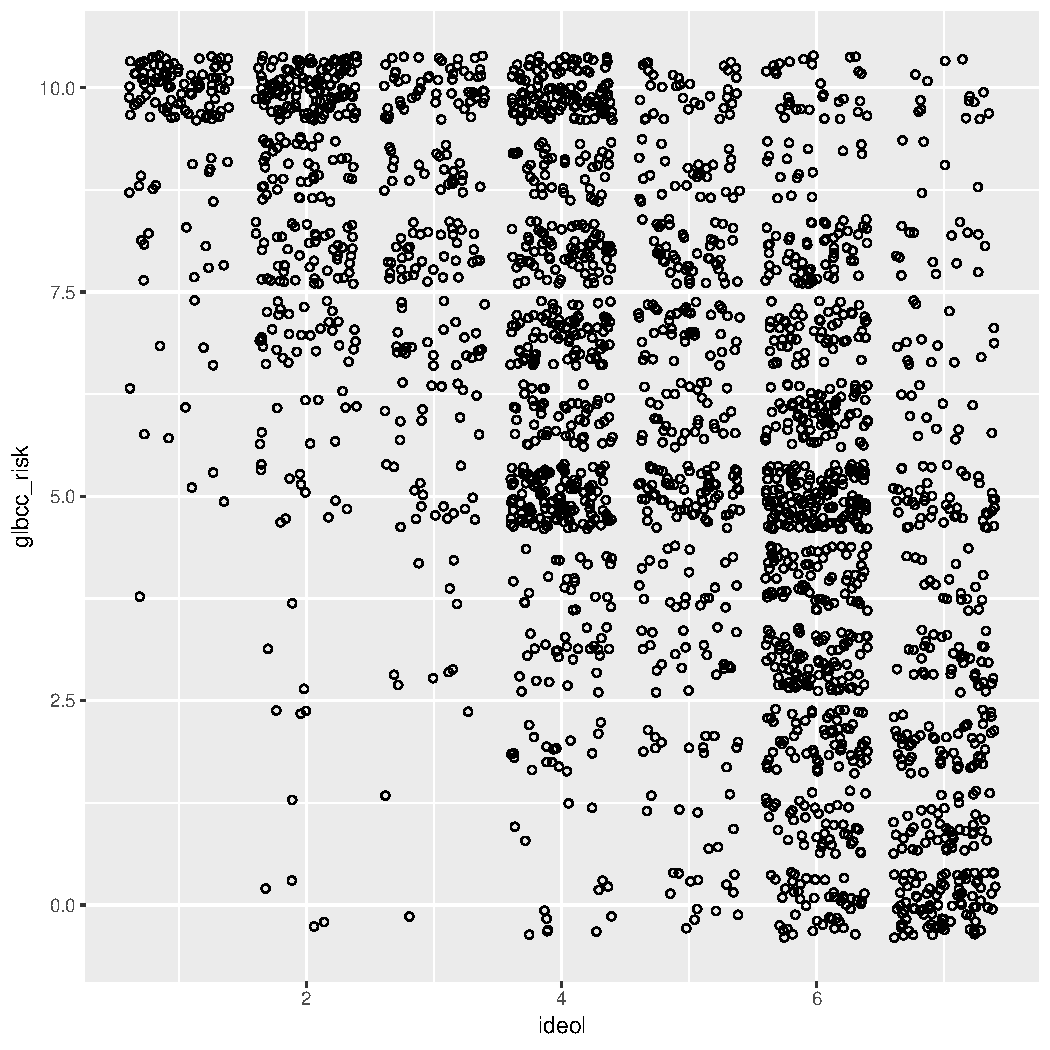
\includegraphics[width=3.5in, height=3.5in]{../06_Association/scatjit.pdf}%filename
\caption{Scatterplot of Ideology and glbcc Risk \label{fig:scatjit}}
\end{figure}   

We can see that the density of values indicate that strong liberals---$1$'s on the ideology scale---tend to view climate change as quite risky, whereas strong conservatives---$7$'s on the ideology scale---tend to view climate change as less risky. Like our previous example, we want to know more about the nature of this relationship. Therefore, we can plot a regression line and a ``loess" line. These lines are the linear and nonlinear estimates of the relationship between political ideology and perceived risk of climate change. We'll have more to say about the linear estimates when we turn to regression analysis in the next chapter. We can add to the previous visualization by including \texttt{geom_smooth} and indicating a "loess" line or an "lm" line. 

% note there is discussion of missing data in the Applied Regression book by Fox - Page 65-67.

\begin{knitrout}
\definecolor{shadecolor}{rgb}{0.969, 0.969, 0.969}\color{fgcolor}\begin{kframe}
\begin{alltt}
\hlstd{ds} \hlopt
  \hlkwd{drop_na}\hlstd{(glbcc_risk, ideol)} \hlopt
  \hlkwd{ggplot}\hlstd{(}\hlkwd{aes}\hlstd{(ideol, glbcc_risk))} \hlopt{+}
  \hlkwd{geom_jitter}\hlstd{(}\hlkwc{shape} \hlstd{=} \hlnum{1}\hlstd{)} \hlopt{+}
  \hlkwd{geom_smooth}\hlstd{(}\hlkwc{method} \hlstd{=} \hlstr{"loess"}\hlstd{,} \hlkwc{color} \hlstd{=} \hlstr{"green"}\hlstd{)} \hlopt{+}
  \hlkwd{geom_smooth}\hlstd{(}\hlkwc{method} \hlstd{=} \hlstr{"lm"}\hlstd{,} \hlkwc{color} \hlstd{=} \hlstr{"red"}\hlstd{)}
\hlkwd{dev.off}\hlstd{()}
\end{alltt}
\end{kframe}
\end{knitrout}

\begin{figure}[!htp]
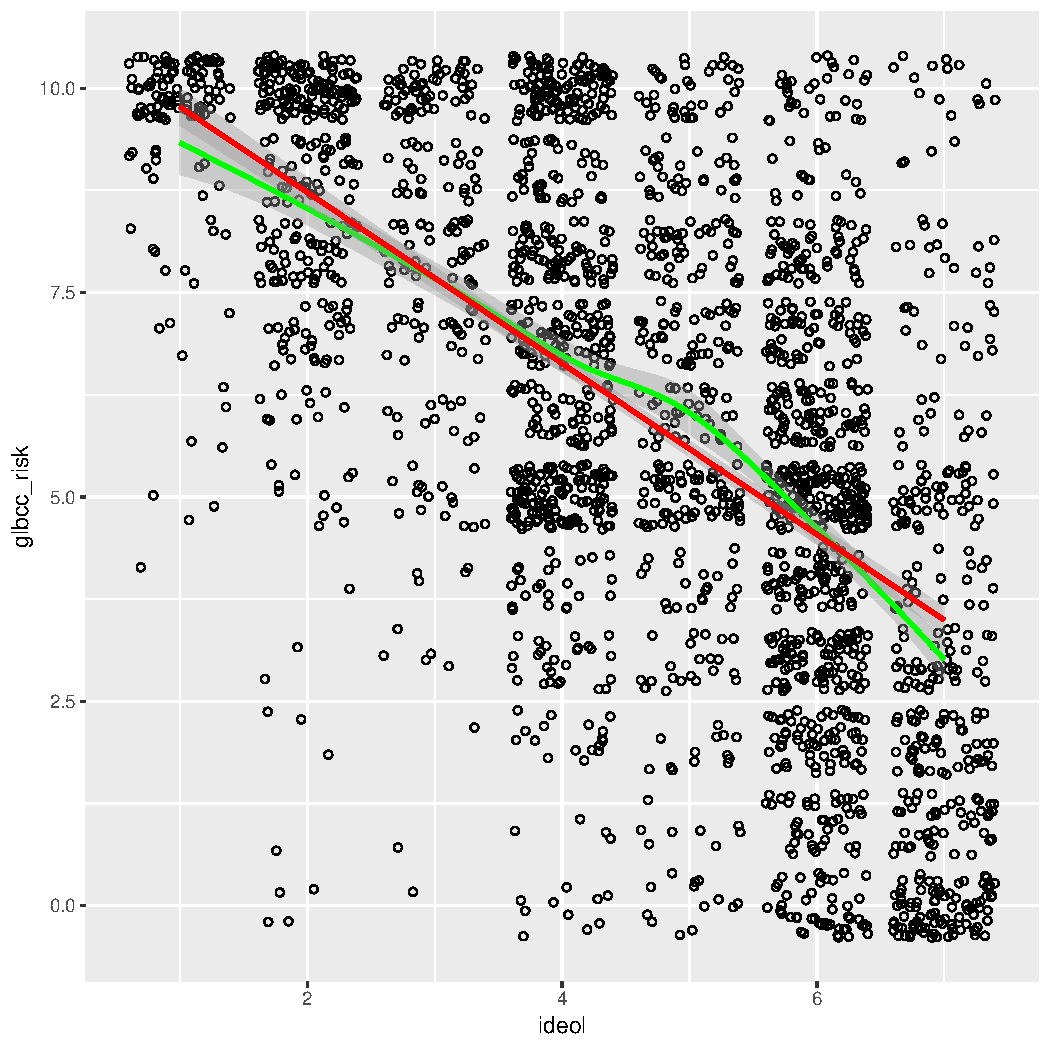
\includegraphics[width=3.5in, height=3.5in]{../06_Association/scatjit2.pdf}%filename
\caption{Scatterplot of Ideology and GLBCC Risk with Regression Line and Lowess Line}
\end{figure}   

Note that the regression lines both slope downward, with average perceived risk  ranging from over 8 for the strong liberals (ideology=1) to less than 5 for strong conservatives (ideology=7). This illustrates how scatterplots can provide information about the nature of the relationship between two variables. We will take the next step -- to bivariate regression analysis -- in the next chapter.

\newpage
% Please add the following required packages to your document preamble:
% \usepackage{graphicx}
\begin{table}[h]
\caption{Appendix 6.1: Chi Square Table}
\label{tab:chisquaretable}
\resizebox{\textwidth}{!}{%
\begin{tabular}{|l|c|c|c|c|c|c|c|c|c|c|c|c|}
\hline
df & \multicolumn{12}{c|}{P-Value} \\ \hline
df & 0.25 & 0.20 & 0.15 & 0.10 & 0.05 & 0.025 & 0.02 & 0.01 & 0.005 & 0.0025 & 0.001 & 0.0005 \\ \hline
1 & 1.32 & 1.64 & 2.07 & 2.71 & 3.84 & 5.02 & 5.41 & 6.63 & 7.88 & 9.14 & 10.83 & 12.12 \\ \hline
2 & 2.77 & 3.22 & 3.79 & 4.61 & 5.99 & 7.38 & 7.82 & 9.21 & 10.60 & 11.98 & 13.82 & 15.20 \\ \hline
3 & 4.11 & 4.64 & 5.32 & 6.25 & 7.81 & 9.35 & 9.84 & 11.34 & 12.84 & 14.32 & 16.27 & 17.73 \\ \hline
4 & 5.39 & 5.59 & 6.74 & 7.78 & 9.49 & 11.14 & 11.67 & 13.23 & 14.86 & 16.42 & 18.47 & 20.00 \\ \hline
5 & 6.63 & 7.29 & 8.12 & 9.24 & 11.07 & 12.83 & 13.33 & 15.09 & 16.75 & 18.39 & 20.51 & 22.11 \\ \hline
6 & 7.84 & 8.56 & 9.45 & 10.64 & 12.53 & 14.45 & 15.03 & 16.81 & 13.55 & 20.25 & 22.46 & 24.10 \\ \hline
7 & 9.04 & 5.80 & 10.75 & 12.02 & 14.07 & 16.01 & 16.62 & 18.48 & 20.28 & 22.04 & 24.32 & 26.02 \\ \hline
8 & 10.22 & 11.03 & 12.03 & 13.36 & 15.51 & 17.53 & 18.17 & 20.09 & 21.95 & 23.77 & 26.12 & 27.87 \\ \hline
9 & 11.39 & 12.24 & 13.29 & 14.68 & 16.92 & 19.02 & 19.63 & 21.67 & 23.59 & 25.46 & 27.83 & 29.67 \\ \hline
10 & 12.55 & 13.44 & 14.53 & 15.99 & 18.31 & 20.48 & 21.16 & 23.21 & 25.19 & 27.11 & 29.59 & 31.42 \\ \hline
11 & 13.70 & 14.63 & 15.77 & 17.29 & 19.68 & 21.92 & 22.62 & 24.72 & 26.76 & 28.73 & 31.26 & 33.14 \\ \hline
12 & 14.85 & 15.81 & 16.99 & 18.55 & 21.03 & 23.34 & 24.05 & 26.22 & 28.30 & 30.32 & 32.91 & 34.82 \\ \hline
13 & 15.93 & 15.58 & 18.90 & 19.81 & 22.36 & 24.74 & 25.47 & 27.69 & 29.82 & 31.88 & 34.53 & 36.48 \\ \hline
14 & 17.12 & 18.15 & 19.4 & 21.06 & 23.68 & 26.12 & 26.87 & 29.14 & 31.32 & 33.43 & 36.12 & 38.11 \\ \hline
15 & 18.25 & 19.31 & 20.60 & 22.31 & 25.00 & 27.49 & 28.26 & 30.58 & 32.80 & 34.95 & 37.70 & 39.72 \\ \hline
16 & 19.37 & 20.47 & 21.79 & 23.54 & 26.30 & 28.85 & 29.63 & 32.00 & 34.27 & 36.46 & 39.25 & 41.31 \\ \hline
17 & 20.49 & 21.61 & 22.98 & 24.77 & 27.59 & 30.19 & 31.00 & 33.41 & 35.72 & 37.95 & 40.79 & 42.88 \\ \hline
18 & 21.60 & 22.76 & 24.16 & 25.99 & 28.87 & 31.53 & 32.35 & 34.81 & 37.16 & 39.42 & 42.31 & 44.43 \\ \hline
19 & 22.72 & 23.90 & 25.33 & 27.20 & 30.14 & 32.85 & 33.69 & 36.19 & 38.58 & 40.88 & 43.82 & 45.97 \\ \hline
20 & 23.83 & 25.04 & 26.50 & 28.41 & 31.41 & 34.17 & 35.02 & 37.57 & 40.00 & 42.34 & 45.31 & 47.50 \\ \hline
21 & 24.93 & 26.17 & 27.66 & 29.62 & 39.67 & 35.48 & 36.34 & 38.93 & 41.40 & 43.78 & 46.80 & 49.01 \\ \hline
22 & 26.04 & 27.30 & 28.82 & 30.81 & 33.92 & 36.78 & 37.66 & 40.29 & 42.80 & 45.20 & 48.27 & 50.51 \\ \hline
23 & 27.14 & 28.43 & 29.98 & 32.01 & 35.17 & 38.08 & 38.97 & 41.64 & 44.18 & 46.62 & 49.73 & 52.00 \\ \hline
24 & 28.24 & 29.55 & 31.13 & 33.20 & 36.42 & 39.36 & 40.27 & 42.98 & 45.56 & 48.03 & 51.18 & 53.48 \\ \hline
25 & 29.34 & 30.68 & 32.28 & 34.38 & 37.65 & 40.65 & 41.57 & 44.31 & 46.93 & 49.44 & 52.62 & 54.95 \\ \hline
26 & 30.43 & 31.79 & 33.43 & 35.56 & 38.89 & 41.92 & 42.86 & 45.64 & 48.29 & 50.83 & 54.05 & 56.41 \\ \hline
27 & 31.53 & 32.91 & 34.57 & 36.74 & 40.11 & 43.19 & 44.14 & 46.96 & 49.64 & 52.22 & 55.48 & 57.86 \\ \hline
28 & 32.62 & 34.03 & 35.71 & 37.92 & 41.34 & 44.46 & 45.42 & 48.28 & 50.99 & 53.59 & 56.89 & 59.30 \\ \hline
29 & 33.71 & 35.14 & 36.85 & 39.09 & 42.56 & 45.72 & 46.69 & 49.59 & 52.34 & 54.97 & 58.30 & 60.73 \\ \hline
30 & 34.80 & 36.25 & 37.99 & 40.26 & 43.77 & 46.98 & 47.96 & 50.89 & 53.67 & 56.33 & 59.70 & 62.16 \\ \hline
40 & 45.62 & 47.27 & 49.24 & 51.81 & 55.76 & 59.34 & 60.44 & 63.69 & 66.77 & 69.70 & 73.40 & 76.09 \\ \hline
50 & 56.33 & 53.16 & 60.35 & 63.17 & 67.50 & 71.42 & 72.61 & 76.15 & 79.49 & 82.66 & 86.66 & 89.56 \\ \hline
60 & 66.98 & 68.97 & 71.34 & 74.40 & 79.08 & 83.30 & 84.58 & 88.38 & 91.95 & 95.34 & 99.61 & 102.7 \\ \hline
80 & 88.13 & 90.41 & 93.11 & 96.58 & 101.9 & 106.6 & 108.1 & 112.3 & 116.3 & 120.1 & 124.8 & 128.3 \\ \hline
100 & 109.1 & 111.7 & 114.7 & 118.5 & 124.3 & 129.6 & 131.1 & 135.8 & 140.2 & 144.3 & 149.4 & 153.2 \\ \hline
\end{tabular}
}
\end{table}
\FloatBarrier
\end{document}
